\documentclass[11pt,preprint]{elsarticle}

\usepackage{lmodern}
%%%% My spacing
\usepackage{setspace}
\setstretch{1.2}
\DeclareMathSizes{12}{14}{10}{10}

% Wrap around which gives all figures included the [H] command, or places it "here". This can be tedious to code in Rmarkdown.
\usepackage{float}
\let\origfigure\figure
\let\endorigfigure\endfigure
\renewenvironment{figure}[1][2] {
    \expandafter\origfigure\expandafter[H]
} {
    \endorigfigure
}

\let\origtable\table
\let\endorigtable\endtable
\renewenvironment{table}[1][2] {
    \expandafter\origtable\expandafter[H]
} {
    \endorigtable
}


\usepackage{ifxetex,ifluatex}
\usepackage{fixltx2e} % provides \textsubscript
\ifnum 0\ifxetex 1\fi\ifluatex 1\fi=0 % if pdftex
  \usepackage[T1]{fontenc}
  \usepackage[utf8]{inputenc}
\else % if luatex or xelatex
  \ifxetex
    \usepackage{mathspec}
    \usepackage{xltxtra,xunicode}
  \else
    \usepackage{fontspec}
  \fi
  \defaultfontfeatures{Mapping=tex-text,Scale=MatchLowercase}
  \newcommand{\euro}{€}
\fi

\usepackage{amssymb, amsmath, amsthm, amsfonts}

\def\bibsection{\section*{References}} %%% Make "References" appear before bibliography


\usepackage[numbers]{natbib}

\usepackage{longtable}
\usepackage[margin=2.3cm,bottom=2cm,top=2.5cm, includefoot]{geometry}
\usepackage{fancyhdr}
\usepackage[bottom, hang, flushmargin]{footmisc}
\usepackage{graphicx}
\numberwithin{equation}{section}
\numberwithin{figure}{section}
\numberwithin{table}{section}
\setlength{\parindent}{0cm}
\setlength{\parskip}{1.3ex plus 0.5ex minus 0.3ex}
\usepackage{textcomp}
\renewcommand{\headrulewidth}{0.2pt}
\renewcommand{\footrulewidth}{0.3pt}

\usepackage{array}
\newcolumntype{x}[1]{>{\centering\arraybackslash\hspace{0pt}}p{#1}}

%%%%  Remove the "preprint submitted to" part. Don't worry about this either, it just looks better without it:
\makeatletter
\def\ps@pprintTitle{%
  \let\@oddhead\@empty
  \let\@evenhead\@empty
  \let\@oddfoot\@empty
  \let\@evenfoot\@oddfoot
}
\makeatother

 \def\tightlist{} % This allows for subbullets!

\usepackage{hyperref}
\hypersetup{breaklinks=true,
            bookmarks=true,
            colorlinks=true,
            citecolor=blue,
            urlcolor=blue,
            linkcolor=blue,
            pdfborder={0 0 0}}


% The following packages allow huxtable to work:
\usepackage{siunitx}
\usepackage{multirow}
\usepackage{hhline}
\usepackage{calc}
\usepackage{tabularx}
\usepackage{booktabs}
\usepackage{caption}


\newenvironment{columns}[1][]{}{}

\newenvironment{column}[1]{\begin{minipage}{#1}\ignorespaces}{%
\end{minipage}
\ifhmode\unskip\fi
\aftergroup\useignorespacesandallpars}

\def\useignorespacesandallpars#1\ignorespaces\fi{%
#1\fi\ignorespacesandallpars}

\makeatletter
\def\ignorespacesandallpars{%
  \@ifnextchar\par
    {\expandafter\ignorespacesandallpars\@gobble}%
    {}%
}
\makeatother


% definitions for citeproc citations
\NewDocumentCommand\citeproctext{}{}
\NewDocumentCommand\citeproc{mm}{%
\href{\#cite.\detokenize{#1}}{#2}\nocite{#1}}

\makeatletter
% allow citations to break across lines
\let\@cite@ofmt\@firstofone
% avoid brackets around text for \cite:
\def\@biblabel#1{}
\def\@cite#1#2{{#1\if@tempswa , #2\fi}}
\makeatother
\newlength{\cslhangindent}
\setlength{\cslhangindent}{1.5em}
\newlength{\csllabelwidth}
\setlength{\csllabelwidth}{3em}
\newenvironment{CSLReferences}[2] % #1 hanging-indent, #2 entry-spacing
{\begin{list}{}{%
	\setlength{\itemindent}{0pt}
	\setlength{\leftmargin}{0pt}
	\setlength{\parsep}{0pt}
	% turn on hanging indent if param 1 is 1
	\ifodd #1
	\setlength{\leftmargin}{\cslhangindent}
	\setlength{\itemindent}{-1\cslhangindent}
	\fi
	% set entry spacing
	\setlength{\itemsep}{#2\baselineskip}}}
{\end{list}}

\usepackage{calc}
\newcommand{\CSLBlock}[1]{\hfill\break\parbox[t]{\linewidth}{\strut\ignorespaces#1\strut}}
\newcommand{\CSLLeftMargin}[1]{\parbox[t]{\csllabelwidth}{\strut#1\strut}}
\newcommand{\CSLRightInline}[1]{\parbox[t]{\linewidth - \csllabelwidth}{\strut#1\strut}}
\newcommand{\CSLIndent}[1]{\hspace{\cslhangindent}#1}


\urlstyle{same}  % don't use monospace font for urls
\setlength{\parindent}{0pt}
\setlength{\parskip}{6pt plus 2pt minus 1pt}
\setlength{\emergencystretch}{3em}  % prevent overfull lines
\setcounter{secnumdepth}{5}

%%% Use protect on footnotes to avoid problems with footnotes in titles
\let\rmarkdownfootnote\footnote%
\def\footnote{\protect\rmarkdownfootnote}
\IfFileExists{upquote.sty}{\usepackage{upquote}}{}

%%% Include extra packages specified by user

%%% Hard setting column skips for reports - this ensures greater consistency and control over the length settings in the document.
%% page layout
%% paragraphs
\setlength{\baselineskip}{12pt plus 0pt minus 0pt}
\setlength{\parskip}{12pt plus 0pt minus 0pt}
\setlength{\parindent}{0pt plus 0pt minus 0pt}
%% floats
\setlength{\floatsep}{12pt plus 0 pt minus 0pt}
\setlength{\textfloatsep}{20pt plus 0pt minus 0pt}
\setlength{\intextsep}{14pt plus 0pt minus 0pt}
\setlength{\dbltextfloatsep}{20pt plus 0pt minus 0pt}
\setlength{\dblfloatsep}{14pt plus 0pt minus 0pt}
%% maths
\setlength{\abovedisplayskip}{12pt plus 0pt minus 0pt}
\setlength{\belowdisplayskip}{12pt plus 0pt minus 0pt}
%% lists
\setlength{\topsep}{10pt plus 0pt minus 0pt}
\setlength{\partopsep}{3pt plus 0pt minus 0pt}
\setlength{\itemsep}{5pt plus 0pt minus 0pt}
\setlength{\labelsep}{8mm plus 0mm minus 0mm}
\setlength{\parsep}{\the\parskip}
\setlength{\listparindent}{\the\parindent}
%% verbatim
\setlength{\fboxsep}{5pt plus 0pt minus 0pt}



\begin{document}



\begin{frontmatter}  %

\title{Riding Offshore Storms: Volatility, Risk Concentration and the
Alpha Opportunity in South African Equities}

% Set to FALSE if wanting to remove title (for submission)




\author[Add1]{Kieron Maseko (26572982)}
\ead{26572982@sun.ac.za}





\address[Add1]{Stellenbosch University, Stellenbosch, South Africa}

\cortext[cor]{Corresponding author: Kieron Maseko (26572982)}

\begin{abstract}
\small{
This report asks whether local equity volatility has risen, how our
flagship SafeCore fund copes with it, and whether stock-pickers have
more room to add value since 2020. Local volatility has not trended up
since 2015, but it comes in episodes, and 2026 is the most volatile year
outside of COVID. It moves closely with global volatility (a GARCH
volatility correlation of 0.85), but the 2026 spike tracks emerging
markets rather than developed markets. In months of high offshore
stress, local volatility runs about a third above normal. SafeCore earns
alpha but does nothing to dampen volatility, and its risk is now
concentrated in gold miners: Resources hold 40\% of the weight but 68\%
of the risk. Dispersion between stocks has recovered to its highest
level since 2022, but in stress periods higher dispersion comes with
higher correlation. We recommend keeping SafeCore's stock-selection edge
while adding a deliberate risk ballast.
}
\end{abstract}

\vspace{1cm}


\begin{keyword}
\footnotesize{
Volatility \sep GARCH \sep DCC \sep Dispersion \sep Factor Exposure \\
\vspace{0.3cm}
}
\footnotesize{
\textit{JEL classification} G11 \sep G12 \sep C58
}
\end{keyword}



\vspace{0.5cm}

\end{frontmatter}

\setcounter{footnote}{0}



%________________________
% Header and Footers
%%%%%%%%%%%%%%%%%%%%%%%%%%%%%%%%%
\pagestyle{fancy}
\chead{}
\rhead{}
\lfoot{}
\rfoot{\footnotesize Page \thepage}
\lhead{}
%\rfoot{\footnotesize Page \thepage } % "e.g. Page 2"
\cfoot{}

%\setlength\headheight{30pt}
%%%%%%%%%%%%%%%%%%%%%%%%%%%%%%%%%
%________________________

\headsep 35pt % So that header does not go over title




\section{\texorpdfstring{Introduction
\label{Introduction}}{Introduction }}\label{introduction}

Offshore shocks have dominated recent markets: tariff wars, record
global policy uncertainty and sharp swings in oil and gold. This report
asks three questions for our investment committee. First, has volatility
on the local exchange increased, and does it simply mirror the global
experience? Second, how well does our flagship fund, SafeCore, handle
that volatility, where does its risk come from, and what factor tilts
does it carry? Third, has the opportunity for active managers to add
value (alpha) improved since 2020, and how does it move with global
conditions?

We follow the standard approach in financial econometrics: measure
volatility in several ways (realised, implied and model-based), test
whether stress regimes change the behaviour of returns, and judge a
portfolio by how it adds up risk, not only by its weights. Section
\ref{Data} describes the data and method, Section \ref{Results} reports
the results for each question, and Section \ref{Conclusion} concludes
with a recommendation.

\section{\texorpdfstring{Data and Methodology
\label{Data}}{Data and Methodology }}\label{data-and-methodology}

We use daily total returns for the Capped SWIX (our benchmark), the Top
40, Mid-cap and Small-cap indexes from 2015, and the MSCI All Country
World (ACWI) and Emerging Markets (EM) indexes as the global comparison
(in USD). Fear gauges include the VIX, V2X and VXEEM implied volatility
indexes, the global Economic Policy Uncertainty index (EPU), the MOVE
bond volatility index, and USD-ZAR implied volatility (SAVIUSD).
SafeCore's monthly holdings are combined with daily stock returns, and
Capped SWIX constituent weights (from August 2020) are used for
dispersion, correlations and factor exposures.

A few data choices matter. Daily stock returns above +50\% or below
-50\% are treated as data errors and removed. SafeCore's weights only
sum to between 79\% and 100\%, so they are rescaled to 100\%. SAVIUSD
contains values recorded divided by 100 between 2021 and 2026, which we
correct. Finally, the official Low-Volatility index only starts in 2024,
so we rebuild it from its constituents back to August 2020; the rebuilt
series has a correlation of 0.999 with the official index over their
common sample.

\textbf{Volatility.} Realised volatility is the annualised standard
deviation of daily returns, \(\sigma = \sqrt{252}\, sd(r_t)\), measured
per calendar year and over a rolling 63-day (three-month) window. To
separate signal from noise we fit an AR(1)-GJR-GARCH(1,1) model with a
skewed-t distribution (\citeproc{ref-bollerslev1986}{Bollerslev, 1986};
\citeproc{ref-glosten1993}{Glosten, Jagannathan \& Runkle, 1993}):

\begin{align}
r_t &= \mu + \phi r_{t-1} + \varepsilon_t, \qquad \varepsilon_t = \sqrt{h_t}\, z_t \notag \\
h_t &= \omega + \alpha \varepsilon_{t-1}^2 + \gamma I_{t-1}\varepsilon_{t-1}^2 + \beta h_{t-1}, \qquad I_{t-1} = 1 \text{ if } \varepsilon_{t-1} < 0 \label{eq1}
\end{align}

Here \(\alpha\) is the impact of a new shock, \(\gamma\) the extra
impact of bad news (the leverage effect) and
\(\alpha + \beta + \gamma/2\) the persistence of volatility. GJR was
chosen over the standard GARCH on information criteria; the more complex
eGARCH and apARCH models improved the fit only marginally.

\textbf{Stratification.} To link local markets to offshore stress, we
flag the months in the top (bottom) 20\% of the VIX, global EPU and
Brent oil volatility. For each index we compare volatility in those
months with its full-sample volatility; a ratio above one means the
index is more volatile in that regime.

\textbf{Portfolio risk.} SafeCore's daily returns are calculated from
its month-end weights, applied from the next trading day. Each stock's
share of portfolio risk is its component contribution to portfolio
volatility, \(w_i (\Sigma w)_i / \sigma_p^2\), using a trailing one-year
covariance matrix at each year-end.

\textbf{Factor scores.} We build our own Momentum score (the six-month
return excluding the latest month) and Low-Volatility score (minus the
six-month realised volatility), standardise both across stocks each
month, and compare them with the third-party scores. A portfolio's
factor exposure is the weighted average score of its holdings.

\textbf{Alpha opportunity.} Dispersion is the weighted cross-sectional
volatility of Capped SWIX constituents:

\begin{align}
CSV_t = \sqrt{\sum_{i} w_{i,t} \left(R_{i,t} - \bar{R}_t\right)^2}, \qquad \bar{R}_t = \sum_i w_{i,t} R_{i,t} \label{eq2}
\end{align}

We weight by index weight because SafeCore is measured against a
cap-weighted benchmark: the alpha it can capture lies where the weight
is, and an unweighted measure lets small, illiquid stocks dominate. We
pair this with the average pairwise correlation of the 40 largest
constituents over a rolling 63-day window, the spread of peer fund
returns, and a DCC-GARCH(1,1) model of the correlations between the
Financials, Industrials and Resources sectors
(\citeproc{ref-engle2002}{Engle, 2002}).

\section{\texorpdfstring{Results
\label{Results}}{Results }}\label{results}

\subsection{Has local volatility increased, and does it mirror the
global
experience?}\label{has-local-volatility-increased-and-does-it-mirror-the-global-experience}

Table \ref{tab1} shows that local volatility has no steady upward trend
since 2015. It comes in episodes: 2015-16, the COVID crash in 2020,
2022, and again in 2026. Even so, 2026 is the most volatile year outside
of COVID for both the Capped SWIX (20.7\%) and the Top 40 (22.4\%). The
local market is also structurally more volatile than the global market,
by about two to six percentage points a year.

\begin{table}[H]
\centering
\caption{Annualised realised volatility (\%) by calendar year (2026 to September) \label{tab1}} 
\begingroup\footnotesize
\begin{tabular}{lrrrrrr}
  \hline
Year & Capped SWIX & Top 40 & MidCaps & SmallCaps & ACWI & EM \\ 
  \hline
2015 & 20.9 & 18.2 & 14.4 & 13.3 & 12.8 & 15.9 \\ 
  2016 & 17.6 & 18.2 & 16.8 & 10.9 & 12.7 & 16.8 \\ 
  2017 & 9.6 & 11.2 & 11.7 & 8.0 & 5.6 & 9.3 \\ 
  2018 & 16.5 & 18.7 & 14.7 & 10.1 & 12.3 & 15.2 \\ 
  2019 & 13.0 & 13.9 & 12.3 & 8.1 & 9.8 & 11.4 \\ 
  2020 & 30.5 & 30.2 & 32.4 & 29.5 & 27.2 & 23.5 \\ 
  2021 & 14.5 & 16.9 & 14.8 & 13.4 & 10.7 & 14.9 \\ 
  2022 & 19.7 & 22.6 & 16.8 & 14.7 & 19.4 & 20.2 \\ 
  2023 & 15.2 & 17.2 & 15.1 & 11.2 & 10.8 & 13.0 \\ 
  2024 & 12.3 & 13.2 & 14.5 & 10.9 & 10.3 & 13.1 \\ 
  2025 & 15.0 & 15.7 & 17.5 & 12.1 & 13.8 & 15.5 \\ 
  2026 & 20.7 & 22.4 & 18.6 & 12.0 & 12.0 & 25.2 \\ 
   \hline
\end{tabular}
\endgroup
\end{table}

\begin{figure}[H]

{\centering 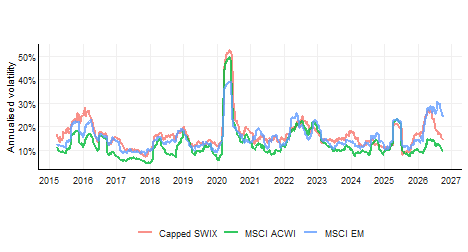
\includegraphics{Question1_files/figure-latex/Figure1-1} 

}

\caption{Rolling three-month realised volatility: local vs global \label{Figure1}}\label{fig:Figure1}
\end{figure}

Figure \ref{Figure1} shows that the big spikes are shared with global
markets, which points to a common driver. The 2026 spike is the
exception: the ACWI stays calm (12.0\% for the year), while MSCI EM
(25.2\%) and the emerging market fear gauge VXEEM (an average of 29.8,
against 18.2 for the VIX) surge. The current rise in local volatility is
therefore an emerging market risk-off event rather than a global one.
With ZAR volatility at its lowest level in the sample, the currency is
not the channel either.

\begin{figure}[H]

{\centering 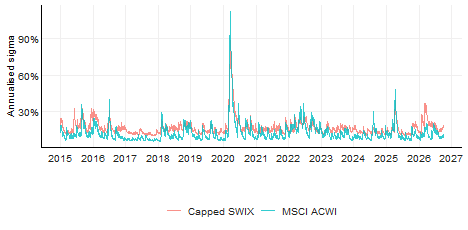
\includegraphics{Question1_files/figure-latex/Figure2-1} 

}

\caption{GJR-GARCH(1,1) conditional volatility (annualised) \label{Figure2}}\label{fig:Figure2}
\end{figure}

The GARCH results confirm this picture. Ljung-Box tests on squared
returns strongly reject the null of no ARCH effects
(\citeproc{ref-engle1982}{Engle, 1982}) (\(p < 0.001\)), which justifies
a volatility model. For the Capped SWIX, \(\beta = 0.90\) and
\(\gamma = 0.13\) are highly significant, while \(\alpha\) is close to
zero: volatility responds to bad news, not good news. Persistence is
high (0.965 locally and 0.973 for the ACWI), so shocks fade slowly. The
standardised residuals show no remaining ARCH effects. The local and
global conditional volatilities in Figure \ref{Figure2} have a
correlation of 0.85.

\begin{table}[H]
\centering
\caption{Volatility in each regime relative to full-sample volatility \label{tab2}} 
\begingroup\footnotesize
\begin{tabular}{lrrrrrr}
  \hline
Period & Capped SWIX & Top 40 & MidCaps & SmallCaps & ACWI & EM \\ 
  \hline
High Global EPU & 1.16 & 1.13 & 1.22 & 1.19 & 1.20 & 1.15 \\ 
  High Oil Vol & 1.30 & 1.25 & 1.18 & 1.19 & 1.28 & 1.26 \\ 
  High VIX & 1.33 & 1.32 & 1.30 & 1.39 & 1.48 & 1.31 \\ 
  Low Global EPU & 1.02 & 0.95 & 0.93 & 0.90 & 0.90 & 0.96 \\ 
  Low Oil Vol & 0.77 & 0.80 & 0.85 & 0.89 & 0.75 & 0.79 \\ 
  Low VIX & 0.76 & 0.76 & 0.83 & 0.73 & 0.53 & 0.70 \\ 
   \hline
\end{tabular}
\endgroup
\end{table}

Table \ref{tab2} shows how offshore stress spills over into local
markets. In high-VIX months, local volatility runs 30-39\% above normal,
and in months of high oil volatility it runs 18-30\% above normal. In
calm months it falls 15-27\% below normal. The link with global policy
uncertainty is weaker (13-22\%), partly because the EPU index has
trended upwards, so its high months cluster in 2025 and 2026. These are
associations, not proof of causation, but they show clearly that
offshore stress changes the risk of holding local equities.

\subsection{How does SafeCore navigate
volatility?}\label{how-does-safecore-navigate-volatility}

\begin{figure}[H]

{\centering 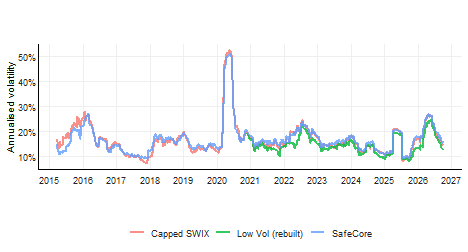
\includegraphics{Question1_files/figure-latex/Figure3-1} 

}

\caption{Rolling three-month volatility: SafeCore, benchmark and Low-Volatility index \label{Figure3}}\label{fig:Figure3}
\end{figure}

SafeCore does not dampen volatility. Figure \ref{Figure3} shows its
volatility sitting on top of the benchmark's throughout, and in 2026 it
is slightly higher (21.1\% against 20.7\%). In high-VIX months its
volatility rises by the same amount as the benchmark's (a ratio of 1.31
against 1.33). Table \ref{tab3} shows that since September 2020 its tail
risk, measured by Value-at-Risk (VaR) and Expected Shortfall (ES), and
its maximum drawdown (18.5\% against 14.1\%) are worse than the
benchmark's.

\begin{table}[H]
\centering
\caption{Risk and return since September 2020 \label{tab3}} 
\begingroup\footnotesize
\begin{tabular}{lrrr}
  \hline
Measure & SafeCore & Capped SWIX & Low Vol (rebuilt) \\ 
  \hline
Annualised return & 0.175 & 0.162 & 0.119 \\ 
  Annualised volatility & 0.169 & 0.164 & 0.149 \\ 
  Sharpe ratio (Rf = 0) & 1.040 & 0.989 & 0.802 \\ 
  Historical VaR (95\%, daily) & -0.017 & -0.016 & -0.015 \\ 
  Modified ES (95\%, daily) & -0.024 & -0.024 & -0.023 \\ 
  Maximum drawdown & 0.185 & 0.141 & 0.150 \\ 
   \hline
\end{tabular}
\endgroup
\end{table}

The fund's strength is returns, not risk control. It has a higher Sharpe
ratio, a beta of 0.95, captures 103\% of the benchmark's up months and
96\% of its down months, and returned more than the benchmark in
high-VIX months. In other words, SafeCore has a benchmark-like risk
profile with a stock-selection edge. The Low-Volatility index shows what
a risk ballast would cost: about 1.5 to 2 percentage points less
volatility, but also about 5\% less return a year over this period.

\begin{figure}[H]

{\centering 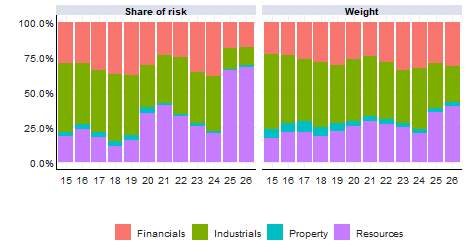
\includegraphics{Question1_files/figure-latex/Figure4-1} 

}

\caption{SafeCore: sector weight vs share of portfolio risk \label{Figure4}}\label{fig:Figure4}
\end{figure}

Figure \ref{Figure4} shows where SafeCore's risk comes from. Until 2019
its risk roughly followed its weights, led by Industrials and
Financials. By August 2026, Resources hold 40\% of the weight but
contribute 68\% of the risk. Three gold and precious metal miners
dominate: AngloGold Ashanti (12\% weight, 28\% of risk), Gold Fields
(7.5\%, 17\%) and Valterra Platinum (4.4\%, 10\%). These stocks are both
volatile and highly correlated with each other, so together they drive
the portfolio. SafeCore has effectively become a single-commodity bet,
which leaves it exposed to exactly the offshore and commodity shocks
identified above.

\begin{table}[H]
\centering
\caption{Average factor exposure (weighted average z-score), August 2020 to August 2026 \label{tab4}} 
\begingroup\footnotesize
\begin{tabular}{lrrrrrr}
  \hline
Factor & Capped SWIX & SafeCore & LowVol & Momentum & Quality & Value \\ 
  \hline
Earnings Quality & -0.00 & 0.13 & -0.06 & 0.00 & 0.05 & 0.16 \\ 
  Growth & -0.03 & 0.02 & -0.06 & 0.01 & 0.09 & -0.02 \\ 
  Momentum & -0.03 & 0.06 & -0.09 & 0.33 & -0.08 & -0.09 \\ 
  Own Low-Vol & 0.32 & 0.34 & 0.54 & 0.31 & 0.35 & 0.26 \\ 
  Own Momentum & 0.12 & 0.21 & 0.06 & 0.34 & 0.08 & 0.10 \\ 
  Value & 0.02 & 0.11 & -0.12 & -0.07 & -0.16 & 0.31 \\ 
  Volatility Sensitivity & -0.04 & -0.03 & -0.01 & -0.10 & 0.02 & -0.08 \\ 
   \hline
\end{tabular}
\endgroup
\end{table}

Table \ref{tab4} places SafeCore's factor exposures next to the
benchmark and four strategy indexes. Relative to the Capped SWIX,
SafeCore leans towards Earnings Quality and Value, has a positive and
recently growing Momentum tilt (as it rides the gold rally), and has no
Low-Volatility tilt. Its Low-Volatility exposure is almost identical to
the benchmark's, and has turned slightly negative in 2026.

Our own Momentum score agrees well with the third-party score (an
average monthly rank correlation of 0.61), so momentum is a robust
signal. Our Low-Volatility score agrees only weakly with the third
party's ``Volatility Sensitivity'' score (0.11). The Low-Volatility
index helps us judge which measure to trust: on our realised-volatility
score it stands far above the benchmark (0.54 against 0.32), but on the
third-party score the two are almost the same. The third-party score
therefore appears to measure something else, such as sensitivity to
market-wide volatility shocks rather than a stock's own volatility. For
a mandate that aims to manage volatility, our realised-volatility score
is the more useful one.

\subsection{Has the alpha opportunity improved since
2020?}\label{has-the-alpha-opportunity-improved-since-2020}

\begin{figure}[H]

{\centering 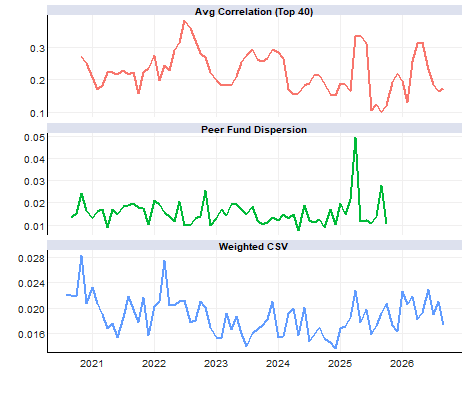
\includegraphics{Question1_files/figure-latex/Figure5-1} 

}

\caption{Measures of the alpha opportunity since 2020 (peer fund data end in October 2025) \label{Figure5}}\label{fig:Figure5}
\end{figure}

Figure \ref{Figure5} tracks the alpha opportunity. Dispersion was
highest in the recovery after COVID. It then fell steadily to a low in
2024, when the average daily weighted CSV was only 1.63\%: correlations
were low, but there was little difference between stocks to exploit.
Since then dispersion has recovered to 2.03\% in 2026, its highest level
since 2022, while correlation remains moderate (0.22). This combination
of stocks moving apart without moving together makes 2026 the best
environment for stock-picking in four years. Weighted and unweighted
dispersion are now almost equal, which shows that the spread is coming
from the large caps, especially the gold miners pulling away from the
rest of the market.

\begin{figure}[H]

{\centering 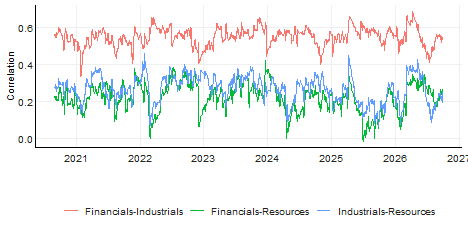
\includegraphics{Question1_files/figure-latex/Figure6-1} 

}

\caption{DCC-GARCH(1,1) conditional correlations between super-sectors \label{Figure6}}\label{fig:Figure6}
\end{figure}

The DCC model in Figure \ref{Figure6} adds a sector view. The
multivariate ARCH test rejects the null of no conditional
heteroskedasticity (\(p < 0.001\)), and the DCC parameters are
significant (\(a = 0.020\), \(b = 0.929\)), so correlations are
time-varying and persistent: a shock to correlations lasts for months,
not days. Financials and Industrials move closely together (around
0.55), as both depend on the domestic economy. Resources are the local
market's diversifier, with correlations of only 0.2 to 0.3 with the
other sectors. This diversification was strongest during the
commodity-led decouplings of 2022 and mid-2025, when sector dispersion,
and so the alpha opportunity, was highest. It weakens during global
stress episodes, when all three correlations rise together.

\begin{table}[H]
\centering
\caption{Alpha-opportunity measures in high and low macro regimes, relative to their average \label{tab5}} 
\begingroup\footnotesize
\begin{tabular}{lrrrrrr}
  \hline
Driver & CSV high & CSV low & Corr. high & Corr. low & Peer disp. high & Peer disp. low \\ 
  \hline
Global EPU & 1.04 & 0.92 & 0.97 & 0.95 & 1.20 & 0.94 \\ 
  MOVE (bond vol) & 1.02 & 1.09 & 1.20 & 0.95 & 1.07 & 1.05 \\ 
  Oil vol & 1.07 & 0.94 & 1.17 & 0.93 & 1.05 & 1.04 \\ 
  VIX & 1.17 & 0.92 & 1.23 & 0.97 & 1.18 & 0.86 \\ 
  ZAR vol & 1.09 & 1.02 & 1.08 & 0.81 & 0.96 & 1.03 \\ 
   \hline
\end{tabular}
\endgroup
\end{table}

Table \ref{tab5} links the alpha opportunity to global conditions. In
high-VIX months dispersion rises by 17\%, but stocks also become 23\%
more correlated. Global stress therefore creates a two-sided
opportunity: there is more to gain from picking the right stocks, but
more of the market moves together, so the gains go to managers who are
positioned correctly on the macro theme. This is why peer fund returns
spread out more when the VIX or global policy uncertainty is high (by
18\% and 20\%). Oil volatility raises both dispersion and correlation,
as commodity shocks split the market into Resources and the rest. Bond
market volatility (MOVE) raises correlation without raising dispersion,
which is the least helpful combination for stock-pickers. The sample is
short (73 months), so these regime effects should be read as indicative.

\section{\texorpdfstring{Conclusion
\label{Conclusion}}{Conclusion }}\label{conclusion}

Local volatility has not risen steadily, but it is high again in 2026,
and it is driven mainly from offshore. It shares its major spikes with
global markets, but the 2026 episode tracks emerging markets, and
periods of high global stress raise local volatility by about a third.
SafeCore has delivered alpha, but it does nothing to dampen this
volatility, and its risk is now concentrated in a handful of gold
miners. The opportunity to add value through stock selection has
improved to its best level since 2022, yet the macro regimes that create
this opportunity are the same ones that make stocks fall together.

We therefore recommend keeping SafeCore's stock-selection process, but
adding a deliberate risk ballast: a cap on the share of risk any one
sector can contribute, a tilt towards low-volatility stocks using our
realised-volatility score, and regular monitoring of offshore stress
indicators such as the VIX, VXEEM and oil volatility. This would let the
fund keep its edge while limiting the damage when global storms reach
local shores.

\newpage

\section*{References}\label{references}
\addcontentsline{toc}{section}{References}

\protect\phantomsection\label{refs}
\begin{CSLReferences}{1}{1}
\bibitem[\citeproctext]{ref-bollerslev1986}
Bollerslev, T. 1986. Generalized autoregressive conditional
heteroskedasticity. \emph{Journal of Econometrics}. 31(3):307--327.

\bibitem[\citeproctext]{ref-engle2002}
Engle, R. 2002. Dynamic conditional correlation: A simple class of
multivariate generalized autoregressive conditional heteroskedasticity
models. \emph{Journal of Business \& Economic Statistics}.
20(3):339--350.

\bibitem[\citeproctext]{ref-engle1982}
Engle, R.F. 1982. Autoregressive conditional heteroscedasticity with
estimates of the variance of united kingdom inflation.
\emph{Econometrica}. 50(4):987--1007.

\bibitem[\citeproctext]{ref-glosten1993}
Glosten, L.R., Jagannathan, R. \& Runkle, D.E. 1993. On the relation
between the expected value and the volatility of the nominal excess
return on stocks. \emph{The Journal of Finance}. 48(5):1779--1801.

\end{CSLReferences}

\bibliography{Tex/ref}





\end{document}
